\documentclass{ximera}

\usepackage{microtype}
\usepackage{tikz}
\usepackage{tkz-euclide}
\usetkzobj{all}
\tikzstyle geometryDiagrams=[ultra thick,color=blue!50!black]

\renewcommand{\epsilon}{\varepsilon}



\title{Central projection}
\begin{document}
\begin{abstract}
Here we start to develop unified models for our geometries.
\end{abstract}
\maketitle

\section{Central projection coordinates}

Let's project $K$-geometry,
\[
1=K\left(x^{2}+y^{2}\right)+z^{2} 
\]
onto the plane $z=1$ using the origin $O=(0,0,0)$ as the center of
projection:
\begin{image}
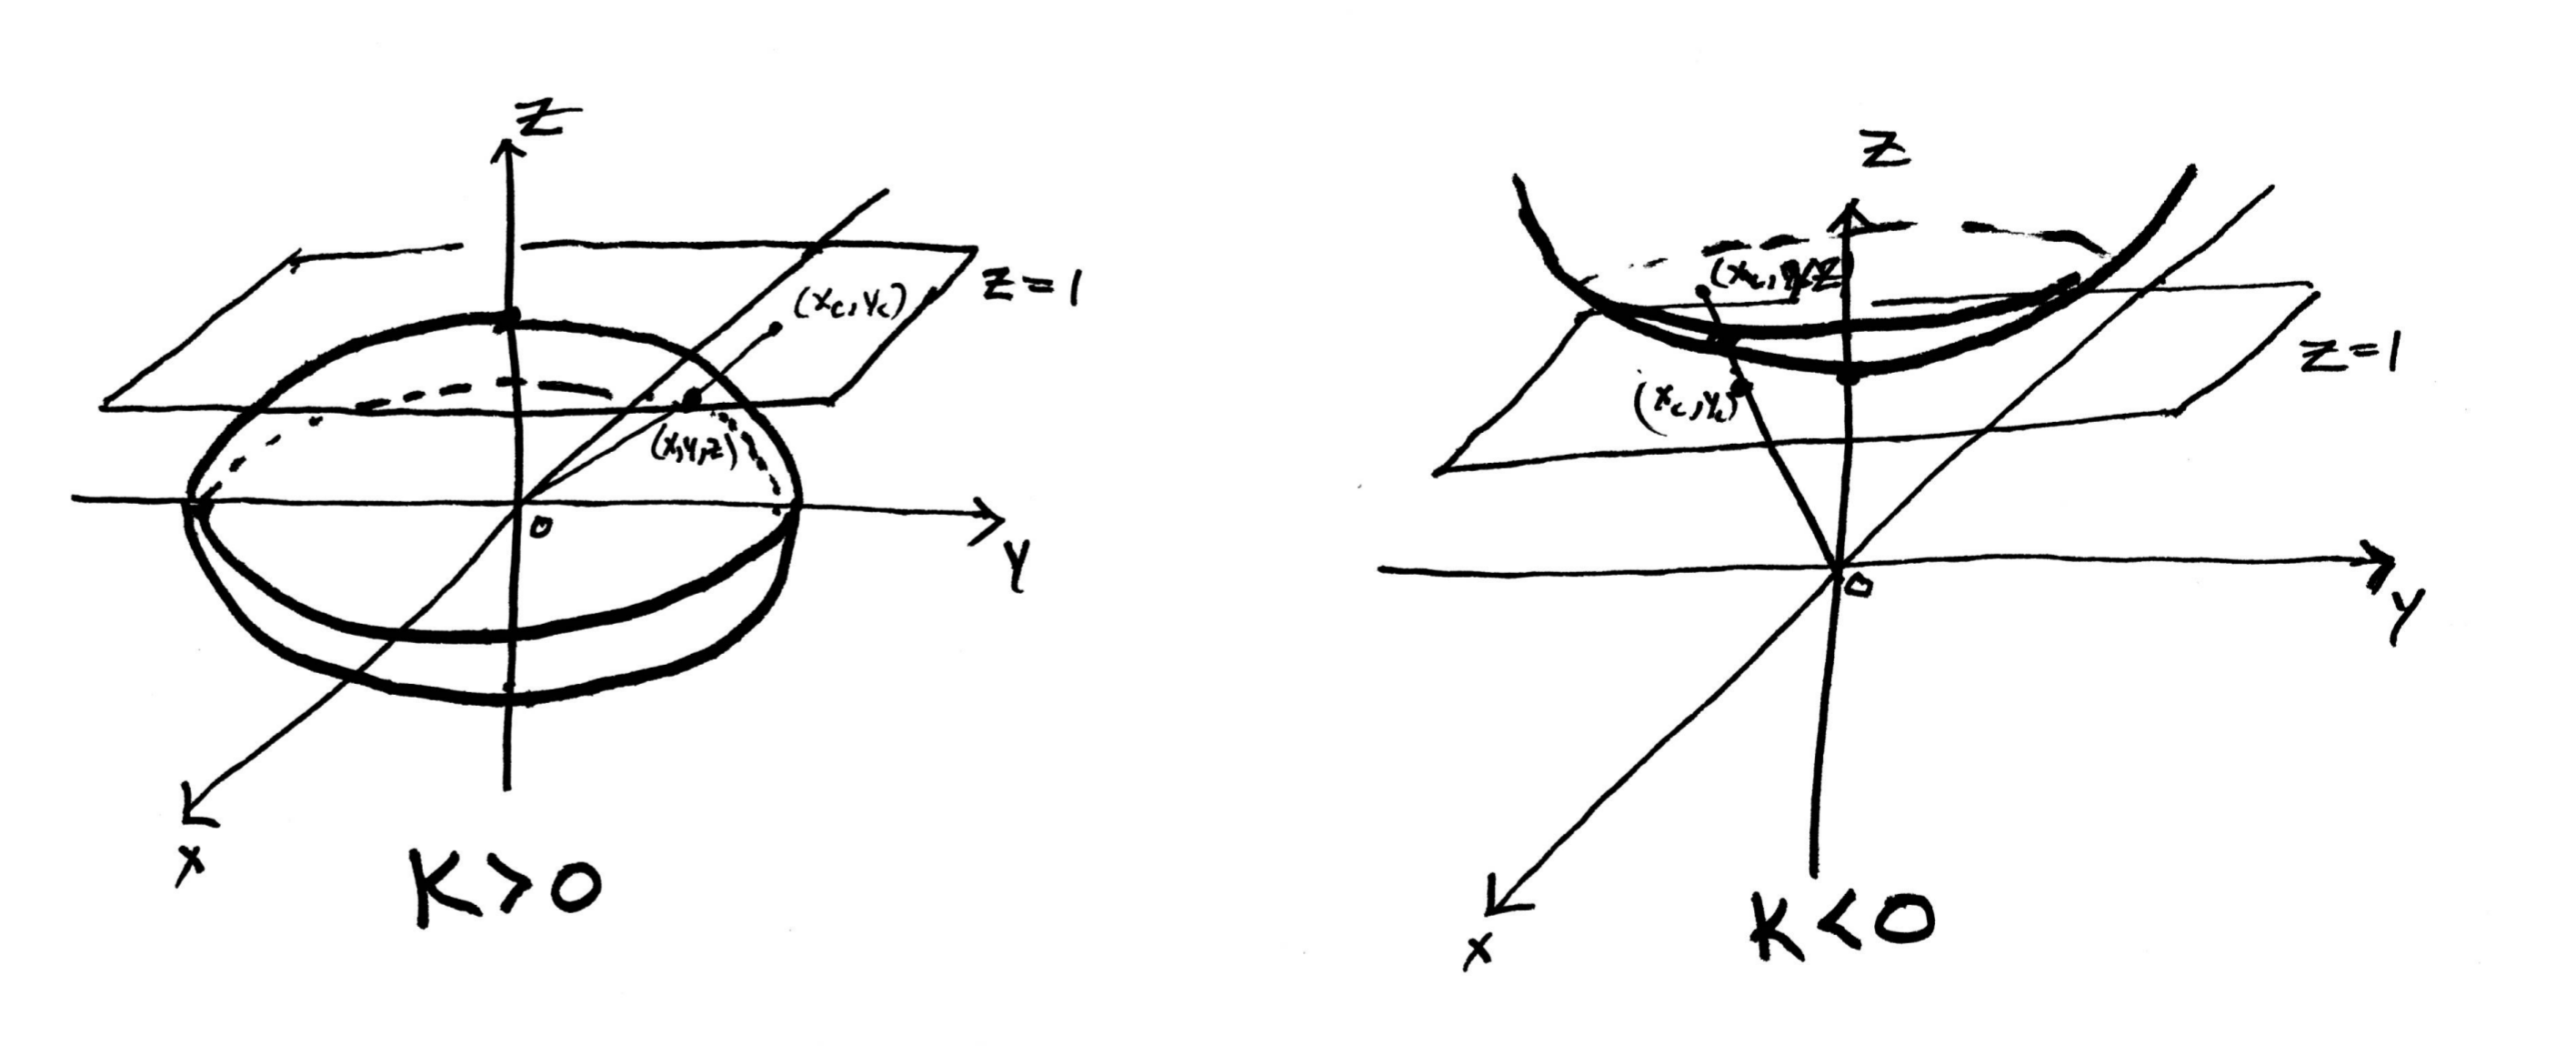
\includegraphics[width=5in]{KGeomCentralProjection.png}
\end{image}
Let's look at this from a different vantage point, say with our eye parallel to the plane $z=1$.
\begin{image}
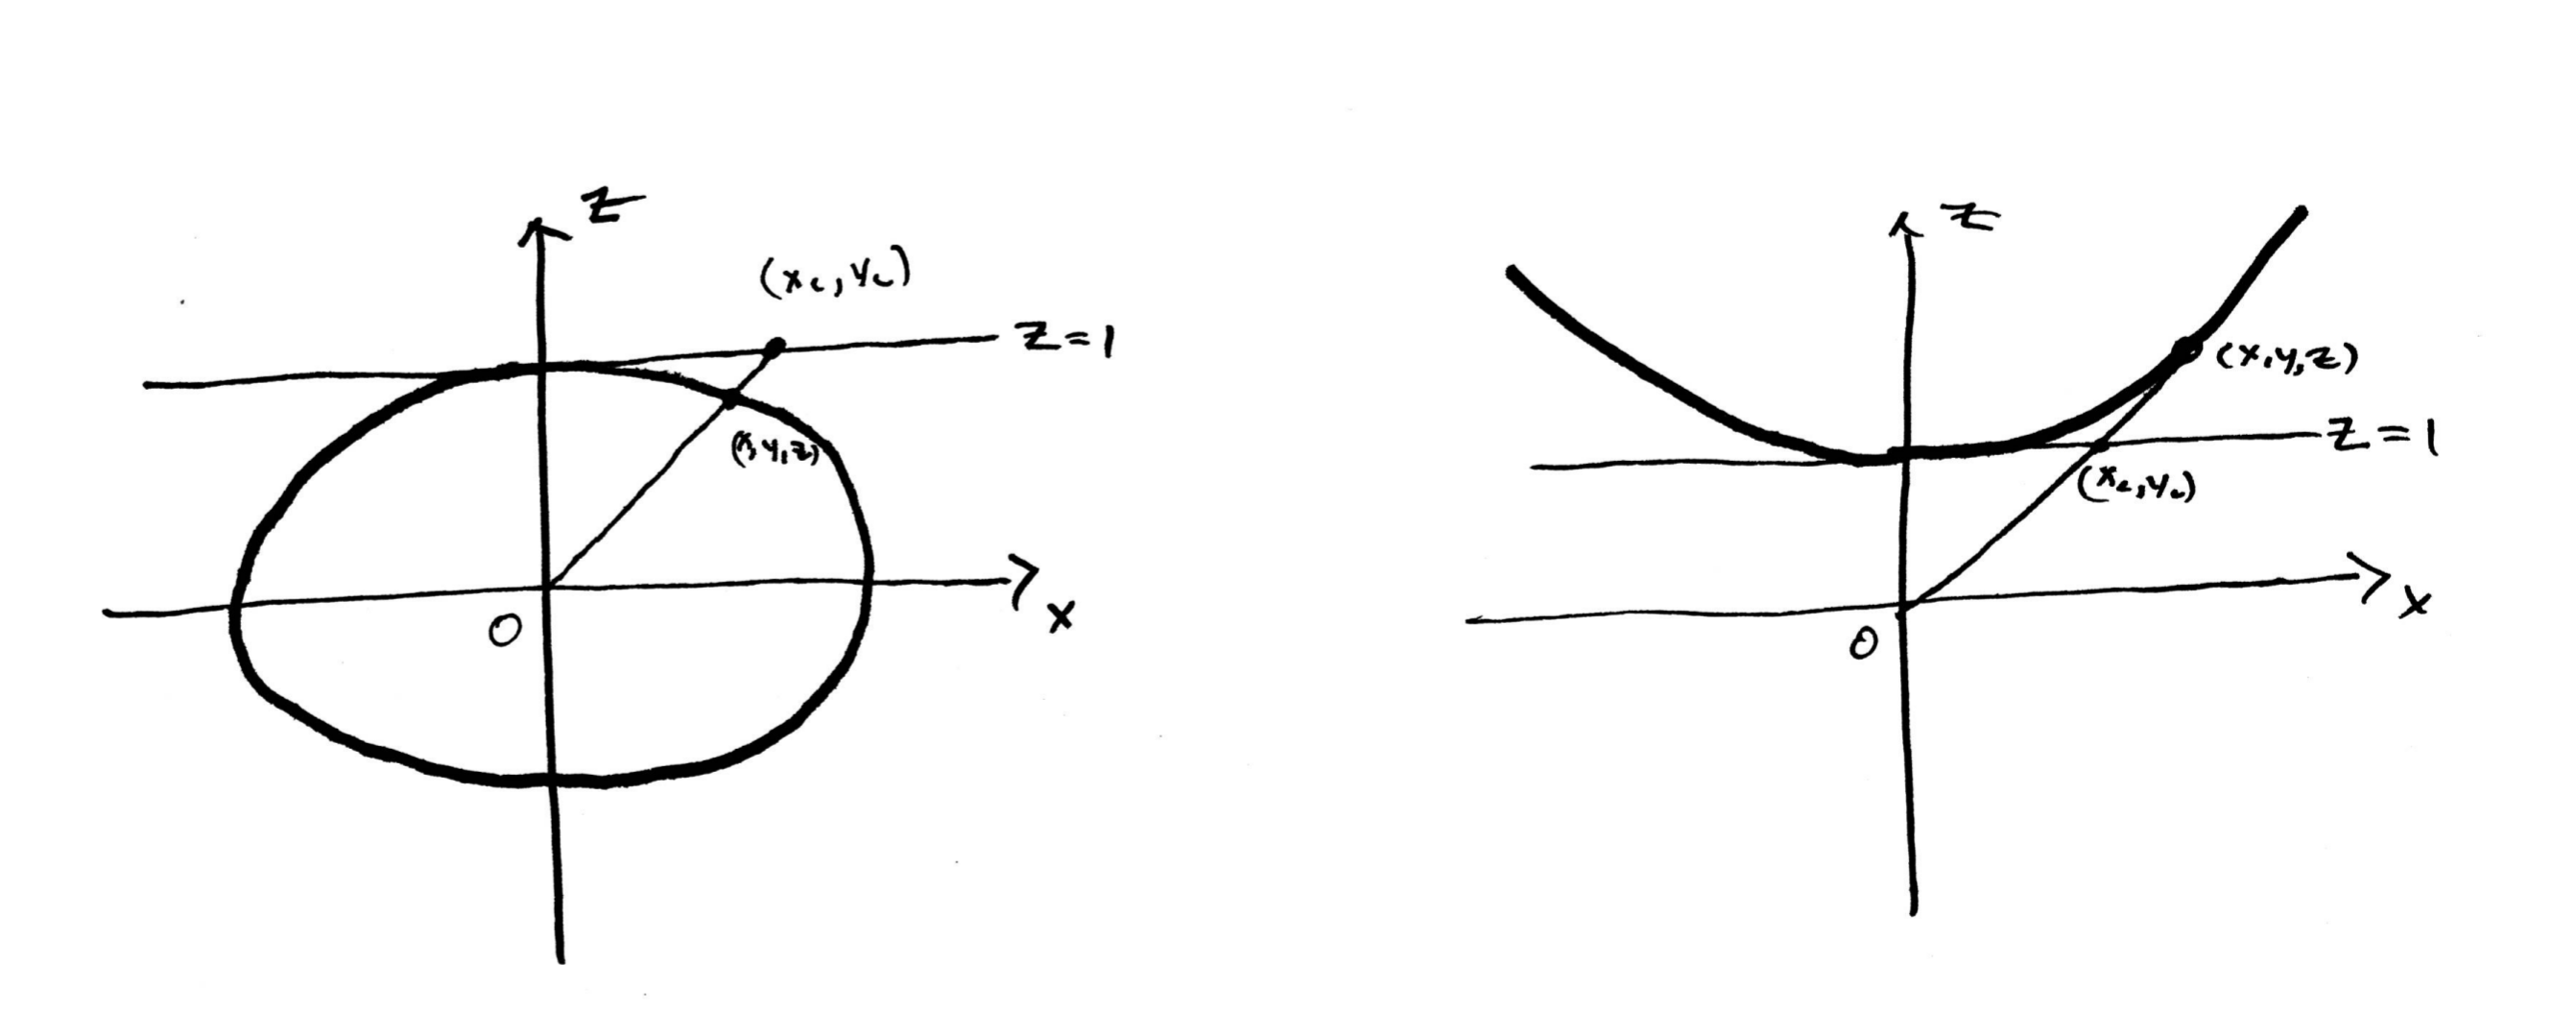
\includegraphics[width=5in]{2dCentralProjection.png}
\end{image}
Note, we are only projecting the top of the surface
\[
1=K\left(x^{2}+y^{2}\right)+z^{2} 
\]
onto the plane $z=1$. So when $K>0$, this is the ``Northern hemisphere'' of
the sphere, when $K<0$, this is the upper hyperboloid, and when $K=0$,
this is the plane $z=1$.

\begin{problem}
  Use similar triangles to explain why there is a number $\lambda$
  such that for any given $(x,y,z)$
  \[
  \lambda\cdot(x_c,y_c,1) = (x,y,z).
  \]
  \begin{freeResponse}
    Let $A = (x,y,z)$, $B= (x,y,0)$, $A_c = (x_c,y_c,1)$ and
    $B_c=(x_c,y_c,0)$. From the diagram above we see that
    \[
    \angle AOB = \angle A_c O B_C.
    \]
    Moreover, since $\triangle AOB$ and $\triangle A_c O B_C$ are
    right triangles, we now see that two of their angles have the same
    measure, and hence all three have the same measure. This means
    that these triangles are similar, and hence there they are
    dilations of one another. Hence there is a scale-factor $\lambda$
    such that
    \[
    \lambda\cdot(x_c,y_c,1) = (x,y,z).
    \]
  \end{freeResponse}
\end{problem}


\begin{problem}
  What range of values could $\lambda$ take when $K>0$?
  \begin{freeResponse}
    In this case, $\lambda\in (0,1)$.
  \end{freeResponse}
\end{problem}

\begin{problem}
  What range of values could $\lambda$ take when $K<0$?
  \begin{freeResponse}
    In this case, $\lambda\in(1,\infty)$.
  \end{freeResponse}
\end{problem}

\begin{problem}
  What range of values could $\lambda$ take when $K=0$?
  \begin{freeResponse}
    In this case
    \[
    1=K\left(x^{2}+y^{2}\right)+z^{2} 
    \]
    is the plane $z = 1$, hence $\lambda=1$.
  \end{freeResponse}
\end{problem}

\begin{problem}
  Letting $(x_c,y_c,1)$ be the image of the $K$-geometry points
  $(x,y,z)$ in the plane $z=1$, use facts about similar triangles to
  explain why
  \[
  \lambda\cdot(x_{c},y_{c},1)=(x,y,z).
  \]
\end{problem}


\begin{problem}
  For the projection of the set $1=K\left(x^{2}+y^{2}\right)+z^{2}$
  onto the $z=1$ plane with center of projection $O$, write
  $(x_{c},y_{c})$ as a function of $(x,y,z)$.
  \begin{freeResponse}
    We know that
    \[
    \lambda\cdot(x_{c},y_{c},1)=(x,y,z),
    \]
    hence $\lambda=z$, and we may now write
    \begin{align*}
      x_{c} &=x/z,\\
      y_{c} &=y/z.
    \end{align*}
  \end{freeResponse}
\end{problem}

\begin{problem}
  For the projection of the set $1=K\left(x^{2}+y^{2}\right)+z^{2} $
  onto the $z=1$ plane with center of projection $O$, write $(x,y,z)$
  as a function of $(x_{c},y_{c})$.
  \begin{freeResponse}
    This is slightly more complex than the previous problem; however,
    we will begin the same way. We know that
    \[
    \lambda\cdot(x_{c},y_{c},1)=(x,y,z),
    \]
    hence $\lambda=z$, and we may now write
    \begin{align*}
      x &= x_c\cdot z,\\
      y &= y_c\cdot z,\\
      z &= z.
    \end{align*}
    Now our task is to write $z$ in terms of $x_c$ and $y_c$. Using our assignments above, write
    \begin{align*}
      1 &= K\left(x^2 + y^2\right) + z^2\\
      1 &= K\left((x_c\cdot z)^2 + (y_c\cdot z)^2\right) + z^2\\
      1 &= \left(K\left(x_c^2 + y_c^2\right)+1\right)z^2,
    \end{align*}
    and so
    \[
    z = \frac{1}{\sqrt{K\left(x_c^2 + y_c^2\right)+1}}.
    \]
    Hence
    \begin{align*}
      x &= \frac{x_c}{\sqrt{K\left(x_c^2 + y_c^2\right)+1}},\\
      y &= \frac{y_c}{\sqrt{K\left(x_c^2 + y_c^2\right)+1}},\\
      z &= \frac{1}{\sqrt{K\left(x_c^2 + y_c^2\right)+1}}.\\
    \end{align*}
  \end{freeResponse}
\end{problem}






\section{Central projection dot product}

Like we have done before, now we want to be able to find a dot product
that will allow us to compute lengths in central projection
coordinates that will agree with the $K$-dot product, and hence the
euclidean dot product.


\begin{problem}
Suppose we have a curve $X$ in $K$-warped space that is a function of
a curve $X_c$ in the plane $z=1$ space. So
\[
X_c(t) = \left( x_c(t),y_c(t)\right)
\]
and
\[
X(t) = 
\begin{cases}
  x(x_c(t),y_c(t)),\\
  y(x_c(t),y_c(t)),\\
  z(x_c(t),y_c(t)).
\end{cases}
\]
Use the chain rule to compute
\[
\dd[x]{t}, \qquad \dd[y]{t}, \qquad \dd[z]{t},
\]
in terms of $\dd[x_c]{t}$, $\dd[y_c]{t}$, $\pp[x]{x_c}$,
$\pp[y]{x_c}$, $\pp[z]{x_c}$, $\pp[x]{y_c}$, $\pp[y]{y_c}$,
and $\pp[z]{y_c}$.
  \begin{hint}
  Simply write down the answer from a previous problem with some minor
  changes.
  \end{hint}
  \begin{freeResponse}
  Write
  \begin{align*}
    \dd[x]{t} &= \left(\pp[x]{x_c},\pp[x]{y_c}\right)\bullet\left(\dd[x_c]{t},\dd[y_c]{t}\right) = \pp[x]{x_c}\cdot\dd[x_c]{t}+\pp[x]{y_c}\cdot\dd[y_c]{t}, \\
    \dd[y]{t} &= \left(\pp[y]{x_c},\pp[y]{y_c}\right)\bullet\left(\dd[x_c]{t},\dd[y_c]{t}\right) = \pp[y]{x_c}\cdot\dd[x_c]{t}+\pp[y]{y_c}\cdot\dd[y_c]{t}, \\
    \dd[z]{t} &= \left(\pp[z]{x_c},\pp[z]{y_c}\right)\bullet\left(\dd[x_c]{t},\dd[y_c]{t}\right) = \pp[z]{x_c}\cdot\dd[x_c]{t}+\pp[z]{y_c}\cdot\dd[y_c]{t}.  
  \end{align*}
\end{freeResponse}
\end{problem}




\begin{problem}
  With the same setting as in the previous problem, rewrite the result
  of your computation in matrix notation to find $D_c$
  such that
\[
\begin{bmatrix}
\dd[x]{t} & \dd[y]{t} & \dd[z]{t}
\end{bmatrix}
=
\begin{bmatrix}
\frac{dx_c}{dt} & \frac{dy_c}{dt}
\end{bmatrix}\cdot D_c.
\]
\begin{hint}
  Simply write down the answer from a previous problem with some minor
  changes.
\end{hint}
\begin{freeResponse}
  \[
  D_c =
  \begin{bmatrix}
    \pp[x]{x_c} & \pp[y]{x_c} & \pp[z]{x_c} \\
    \pp[x]{y_c}   & \pp[y]{y_c}   & \pp[z]{y_c}
  \end{bmatrix}.
  \]
\end{freeResponse}
\end{problem}




\begin{problem}
  Now find $P_c$ in terms of $K$, $\pp[x]{x_c}$, $\pp[y]{x_c}$,
  $\pp[z]{x_c}$, $\pp[x]{y_c}$, $\pp[y]{y_c}$, and $\pp[z]{y_c}$ such
  that
  \[
  \left(\dd[x]{t}, \dd[y]{t}, \dd[z]{t}\right)\bullet_K
  \left(\dd[x]{t}, \dd[y]{t}, \dd[z]{t}\right)
  =
  \begin{bmatrix}
    \dd[x_c]{t} &  \dd[y_c]{t}
  \end{bmatrix}
  \cdot P_c
  \cdot
  \begin{bmatrix}
    \dd[x_c]{t} \\  \dd[y_c]{t}
  \end{bmatrix}.
  \]
  \begin{hint}
  Simply write down the answer from a previous problem with some minor
  changes.
  \end{hint}
  \begin{freeResponse}
    For completeness sake, we will include a complete solution.
    Working from the $K$-dot product, we need that
    \begin{align*}
    \left(\dd[x]{t}, \dd[y]{t}, \dd[z]{t}\right)\bullet_K
    \left(\dd[x]{t}, \dd[y]{t}, \dd[z]{t}\right)
    &=
    \begin{bmatrix}
      \dd[x]{t} & \dd[y]{t} & \dd[z]{t}
    \end{bmatrix}
    \begin{bmatrix}
      1 & 0 & 0\\
      0 & 1 & 0\\
      0 & 0 & K^{-1}
    \end{bmatrix}
    \begin{bmatrix}
      \dd[x]{t} \\ \dd[y]{t} \\ \dd[z]{t}
    \end{bmatrix}\\
    &=
    \begin{bmatrix}
      \frac{dx_c}{dt} & \frac{dy_c}{dt}
    \end{bmatrix}\cdot D_{c}\cdot
    \begin{bmatrix}
      1 & 0 & 0\\
      0 & 1 & 0\\
    0 & 0 & K^{-1}
    \end{bmatrix}
    \cdot
    \left(
    \begin{bmatrix}
      \frac{dx_c}{dt} & \frac{dy_c}{dt}
    \end{bmatrix}\cdot D_{c}
    \right)^\transpose\\
    &=
    \begin{bmatrix}
      \frac{dx_c}{dt} & \frac{dy_c}{dt}
    \end{bmatrix}\cdot D_{c}\cdot
    \begin{bmatrix}
      1 & 0 & 0\\
      0 & 1 & 0\\
    0 & 0 & K^{-1}
    \end{bmatrix}
    \cdot
    D_{c}^\transpose
    \cdot \begin{bmatrix}
      \frac{dx_c}{dt} \\ \frac{dy_c}{dt}
    \end{bmatrix}.
  \end{align*}
    Hence
    \begin{align*}
      P_c &=
      \begin{bmatrix}
        \pp[x]{x_c} & \pp[y]{x_c} & \pp[z]{x_c} \\
        \pp[x]{y_c} & \pp[y]{y_c} & \pp[z]{y_c}
      \end{bmatrix}
      \begin{bmatrix}
        1 & 0 & 0\\
        0 & 1 & 0\\
        0 & 0 & K^{-1}
      \end{bmatrix}
      \begin{bmatrix}
        \pp[x]{x_c} & \pp[x]{y_c}\\ 
        \pp[y]{x_c} & \pp[y]{y_c}\\
        \pp[z]{x_c} & \pp[z]{y_c}
      \end{bmatrix}\\
      &=
      \begin{bmatrix}
        \left(\pp[x]{x_c}\right)^2 + \left(\pp[y]{x_c}\right)^2 + \left(\pp[z]{x_c}\right)^2K^{-1} & \pp[x]{x_c}\pp[x]{y_c} + \pp[y]{x_c}\pp[y]{y_c} + \pp[z]{x_c}\pp[z]{y_c} K^{-1}\\
        \pp[x]{x_c}\pp[x]{y_c} + \pp[y]{x_c}\pp[y]{y_c} + \pp[z]{x_c}\pp[z]{y_c} K^{-1}       & \left(\pp[x]{y_c}\right)^2 + \left(\pp[y]{y_c}\right)^2 + \left(\pp[z]{y_c}\right)^2K^{-1}
      \end{bmatrix}.
    \end{align*}
  \end{freeResponse}
\end{problem}

Before we actually compute $P_c$, it will help to compute the partial
derivatives.

\begin{problem}
  Set
  \begin{align*}
    x(x_c,y_c) &=x/\lambda,\\
    y(x_c,y_c) &=y/\lambda,\\
    z(x_c,y_c) &=\lambda,
  \end{align*}
  and show that
  \[
  \begin{split}
    \pp[x]{x_c} &=\lambda -Kx_c^2 \lambda^3,\\
    \pp[y]{x_c} &=-Kx_cy_c \lambda^3,\\
    \pp[z]{x_c} &=-Kx_c \lambda^3,
  \end{split}
  \qquad
  \begin{split}
    \pp[x]{y_c} &= -Kx_cy_c \lambda^3,\\
    \pp[y]{y_c} &= \lambda - Ky_c^2 \lambda^3,\\
    \pp[z]{y_c} &= -Ky_c \lambda^3.
  \end{split}
  \]
  \begin{hint}
  Work in the following way:
  \begin{enumerate}
  \item Recall $x = \lambda\cdot x_c$.
  \item Note that $\pp[x]{x_c} = \lambda + x_c \cdot \pp[\lambda]{x_c}$.
    \item Express the partial derivative in terms of $\lambda$, $K$, $x_c$,
      and $y_c$.
  \end{enumerate}
\end{hint}
  \begin{freeResponse}
    Write
  \begin{align*}
    \pp[x]{x_c} &= \lambda  + x_c \cdot \pp[\lambda]{x_c}\\
    &= \lambda + x_c \cdot \pp{x_c} \left(K\left(x_c^2 + y_c^2\right)+1\right)^{-1/2}\\
    &= \lambda + x_c \cdot (-1/2)\left(K\left(x_c^2 + y_c^2\right)+1\right)^{-3/2}(2Kx_c)\\
    &= \lambda -Kx_c^2 \lambda^3.
  \end{align*}
  Similarly,
    \begin{align*}
    \pp[y]{x_c} &= y_c \cdot \pp[\lambda]{x_c}\\
    &= y_c \cdot \pp{x_c} \left(K\left(x_c^2 + y_c^2\right)+1\right)^{-1/2}\\
    &= y_c \cdot (-1/2)\left(K\left(x_c^2 + y_c^2\right)+1\right)^{-3/2}(2Kx_c)\\
    &= -Kx_cy_c \lambda^3.
    \end{align*}
   Finally, 
    \begin{align*}
    \pp[z]{x_c} &= \pp[\lambda]{x_c}\\
    &= \pp{x_c}\left(K\left(x_c^2 + y_c^2\right)+1\right)^{-1/2}\\
    &= (-1/2)\left(K\left(x_c^2 + y_c^2\right)+1\right)^{-3/2}(2Kx_c)\\
    &= -Kx_c \lambda^3.
    \end{align*}
    Now with entirely similar computations, we see
    \begin{align*}
      \pp[x]{y_c} &= -Kx_cy_c \lambda^3,\\
      \pp[y]{y_c} &= \lambda - Ky_c^2 \lambda^3,\\
      \pp[z]{y_c} &= -Ky_c \lambda^3.
    \end{align*}
  \end{freeResponse}
\end{problem}



\begin{problem}
With the same setting as above, show that $P_c$ is
  \[
  P_c =
  \begin{bmatrix}
    \left(Ky_c^2+1\right)\lambda^4 & -Kx_{c}y_{c}\lambda^4\\
    -Kx_{c}y_{c}\lambda^4 & \left(Kx_c^2+1\right)\lambda^4
  \end{bmatrix}.
\]

\begin{hint}
  When simplifying, combine the terms with the highest degree of $\lambda$
  and note that
  \[
  \lambda^{-2} = K\left(x_c^2 + y_c^2\right) + 1.
  \]
\end{hint}
\begin{freeResponse}
  
  Write $\left(\pp[x]{x_c}\right)^2 + \left(\pp[y]{x_c}\right)^2 +\left(\pp[z]{x_c}\right)^2K^{-1}$
    \begin{align*}
      &= \left(\lambda -Kx_c^2 \lambda^3\right)^2 + \left(-Kx_cy_c \lambda^3\right)^2 + \left(-Kx_c \lambda^3\right)^2K^{-1}\\
      &= \lambda^2 - 2Kx_c^2\lambda^4 + K^2x_c^4 \lambda^6+ K^2x_c^2y_c^2\lambda^6 + Kx_c^2\lambda^6\\
      &= \lambda^2 - 2Kx_c^2\lambda^4 + Kx_c^2\lambda^6\left(Kx_c^2 + Ky_c^2 + 1\right)\\
      &= \lambda^2 - 2Kx_c^2\lambda^4 + Kx_c^2\lambda^6\left(K\left(x_c^2 + y_c^2\right) + 1\right)\\
      &= \lambda^2 - 2Kx_c^2\lambda^4 + Kx_c^2\lambda^6 \lambda^{-2}\\
      &= \lambda^2 - 2Kx_c^2\lambda^4 + Kx_c^2\lambda^4\\
      &= \lambda^2 - Kx_c^2\lambda^4\\
      &= \frac{1}{K\left(x_c^2+y_c^2\right)+1} - \frac{Kx_c^2}{\left(K\left(x_c^2+y_c^2\right)+1\right)^2}\\
      &= \frac{K\left(x_c^2 + y_c^2\right) +1 - Kx_c^2}{\left(K\left(x_c^2+y_c^2\right)+1\right)^2}\\
      &= \frac{Ky_c^2+1}{\left(K\left(x_c^2+y_c^2\right)+1\right)^2}\\
      &= \left(Ky_c^2+1\right)\lambda^4.
    \end{align*}
    
    That $\pp[x]{x_c}\pp[x]{y_c} + \pp[y]{x_c}\pp[y]{y_c} + \pp[z]{x_c}\pp[z]{y_c} K^{-1}$
    \begin{align*}
      &=\left(\lambda -Kx_c^2 \lambda^3\right)\left(-Kx_cy_c \lambda^3\right) + \left(-Kx_cy_c \lambda^3\right)\left(\lambda - Ky_c^2 \lambda^3\right) + \left(-Kx_c \lambda^3\right)\left(-Ky_c \lambda^3\right)K^{-1}\\
      &= -Kx_cy_c\lambda^4+K^2x_c^3y_c\lambda^6-Kx_cy_c\lambda^4+K^2x_cy_c^3\lambda^6+Kx_cy_c\lambda^6\\
      &= K^2x_c^3y_c\lambda^6+K^2x_cy_c^3\lambda^6+Kx_cy_c\lambda^6 -2Kx_cy_c\lambda^4\\
      &= Kx_cy_c\lambda^6\left(K\left(x_c^2 + y_c^2\right) + 1\right)-2Kx_cy_c\lambda^4\\
      &= Kx_cy_c\lambda^6\lambda^{-2} -2Kx_cy_c\lambda^4\\
      &= Kx_cy_c\lambda^4 -2Kx_cy_c\lambda^4\\
      &= -Kx_cy_c\lambda^4.
    \end{align*}
    With entirely analogous computations, we see that 
    \[
     P_c =
     \begin{bmatrix}
       \left(Ky_c^2+1\right)\lambda^4 & -Kx_{c}y_{c}\lambda^4\\
       -Kx_{c}y_{c}\lambda^4 & \left(Kx_c^2+1\right)\lambda^4
     \end{bmatrix}.
     \]
  \end{freeResponse}
\end{problem}


\begin{definition}
  Let $V_c$ and $W$ be a vectors in $(x_c,y_c)$-coordinates
  originating at the same $(x_c,y_c)$-coordinate. Define
  \[
  V_c \bullet_c W_c = V_c \cdot P_c \cdot W_c^\transpose
  \]
  where
  \[
  P_c =
  \begin{bmatrix}
    \left(Ky_c^2+1\right)\lambda^4 & -Kx_{c}y_{c}\lambda^4\\
    -Kx_{c}y_{c}\lambda^4 & \left(Kx_c^2+1\right)\lambda^4
  \end{bmatrix}
  \]
  and $\lambda$, $x_c$, and $y_c$ are determined by the
  coordinate that the vectors originate from.
\end{definition}


\section{When the finite is infinite and the infinite is finite}

Central projection allows us to think about both ``finite'' areas and
``infinite'' areas in new ways.

\paragraph{When $K$ is positive, the finite is infinite}

When $K>0$, we are working with a sphere. As we know, a sphere has
finite surface area.

\begin{problem}
  As a point approaches the equator of the $R$-sphere from the North
  Pole, where does it move to under central projection?
  \begin{hint}
    A picture is worth a thousand words!
  \end{hint}
  \begin{freeResponse}
  \end{freeResponse}
\end{problem}

\begin{problem}
  Explain why one might say that central projection makes the
  ``finite'' seem ``infinite.''
    \begin{freeResponse}
    \end{freeResponse}
\end{problem}


\paragraph{When $K$ is negative, the infinite is finite}


Notice that, if $K<0$, the equation of $K$-geometry becomes
\[
z^{2}-|K|\left(x^{2}+y^{2}\right)  =1.
\]
This describes a $K$-geometry forms a $2$-sheeted hyperboloid with the
$z$-axis as major axis. We will only consider the sheet on which $z$
is positive as forming the $K$-geometry. In plain English, this means
we are doing geometry on this hyperboloid:
\begin{image}
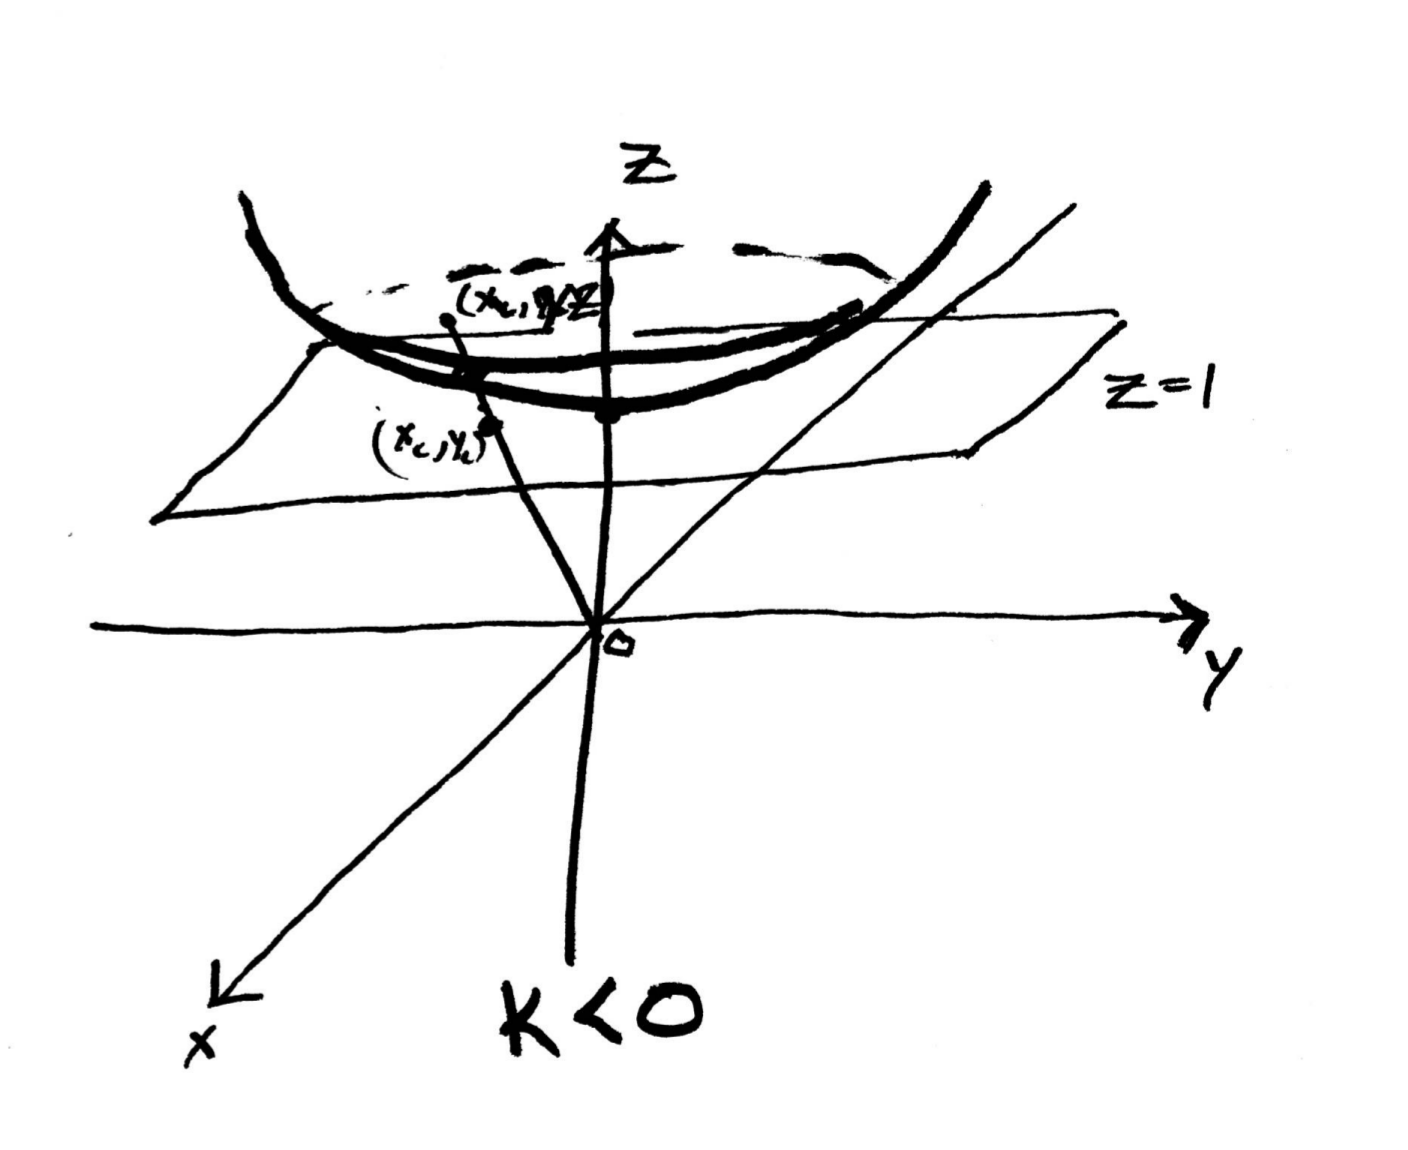
\includegraphics[width=3in]{UpperHyperboloid.png}
\end{image}
Of critical importance, note

\begin{center}
  \textbf{this hyperboloid has infinite surface area.}
\end{center}

The hyperboloid above is obtained by rotating the hyperbola
\[
z^{2}-\left\vert K\right\vert x^{2}= 1
\]
in the $(x,z)$-plane around the $z$-axis.
\begin{image}
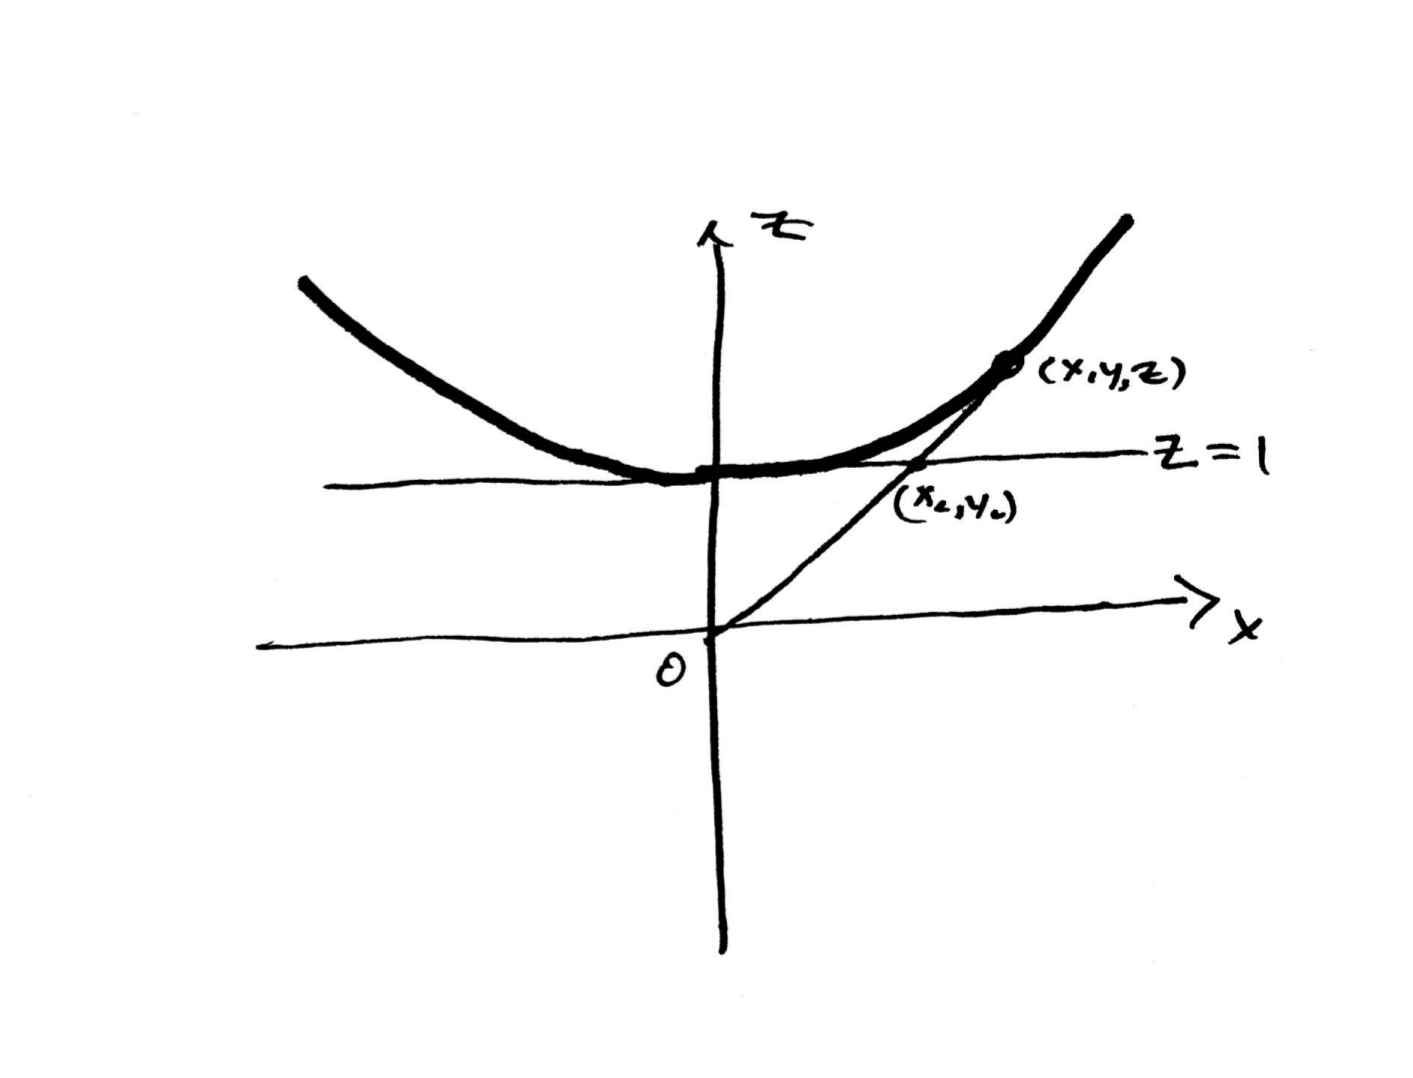
\includegraphics[width=3in]{UpperHyperbola.png}
\end{image}


\begin{problem}
  Compute the (slant) asymptotes of the curve
  \[
  z^{2}-\left\vert K\right\vert x^{2}= 1
  \]
  \begin{hint}
    First rewrite $z^{2}-|K|x^{2} =1$ as
    \[
    z = \sqrt{1+|K|x^2}
    \]
    and explain why this is acceptable.
  \end{hint}
  \begin{hint}
    Explain why computing this limit
    \[
    \lim_{x\to \infty} \frac{\sqrt{1+|K|x^2}}{x}
    \]
    helps us compute (one) of the asymptotes.
  \end{hint}
  \begin{freeResponse}
    Since we are only considering the upper hyperboloid, we need only
    look at the upper hyperbola. Hence we may look at
     \[
    z = \sqrt{1+|K|x^2}.
    \]
    To compute the slope of one of the asymptotes of this curve,
    compute
    \[
    \lim_{x\to \infty} \frac{\sqrt{1+|K|x^2}}{x}
    \]
    as this computes the ``end-behavior'' of the ``slope'' of the
    curve. Write
    \begin{align*}
      \lim_{x\to \infty} \frac{\sqrt{1+|K|x^2}}{x} &= \lim_{x\to \infty} \frac{\sqrt{1+|K|x^2}}{x}\cdot \frac{1/x}{1/x}\\
      &= \lim_{x\to \infty} \sqrt{1/x^2+|K|}\\
      &= \sqrt{|K|}.
    \end{align*}
    Hence one asymptote is given by $z = x\sqrt{|K|}$. To compute the other asymptote, write
    \begin{align*}
      \lim_{x\to -\infty} \frac{\sqrt{1+|K|x^2}}{x} &= \lim_{x\to \infty} \frac{\sqrt{1+|K|x^2}}{x}\cdot \frac{1/(-x)}{1/(-x)}\\
      &= \lim_{x\to \infty} -\sqrt{1/x^2+|K|}\\
      &= -\sqrt{|K|}.
    \end{align*}
    Hence the other asymptote is given by $z = -x\sqrt{|K|}$.
  \end{freeResponse}
\end{problem}


Rotating the asymptotes in the $(x,z)$-plane around the $z$-axis gives
us the \textit{asymptotic cone}.  The central projection coordinates
$(x_{c},y_{c})$ of $K$-geometry when $K<0$ only correspond to points
in $K$-geometry when $(x_{c},y_{c},1)$ lies \textit{inside} the
asymptotic cone.

\begin{problem}
  When $K<0$, find the radius of the disk in the plane $z=1$ whose
  perimeter is determined by the asymptotic cone. 
  \begin{hint}
    Work with the asymptote(s) you found above.
  \end{hint}
  \begin{freeResponse}
    We must find where $z = x\sqrt{|K|}$ intersects the line $z=1$. To do this, simply solve
    \[
    1 = x\sqrt{|K|}
    \]
    for $x$, and so the radius is $1/\sqrt{|K|}$.
  \end{freeResponse}
\end{problem}

\begin{problem}
  Explain why one might say that central projection makes the
  ``infinite'' seem ``finite.''
    \begin{freeResponse}
    \end{freeResponse}
\end{problem}


\begin{problem}
  When $K<0$, what happens to the radius of disk determined by central
  projection as $K$ goes to infinity. Explain why this makes perfect
  sense.
\end{problem}




\begin{problem}
Summarize the results from this section. In particular, indicate which
results follow from the others.
\begin{freeResponse}
\end{freeResponse}
\end{problem}


\end{document}
